\documentclass[tikz,border=9pt]{standalone}
\usepackage{amsmath}
\usetikzlibrary{arrows.meta,calc,decorations.pathmorphing}
\definecolor{ink}{HTML}{21352F}
\definecolor{teal}{HTML}{087F7B}
\definecolor{blue}{HTML}{4B77A8}
\definecolor{gold}{HTML}{C58B2A}
\definecolor{rose}{HTML}{B65A62}
\begin{document}
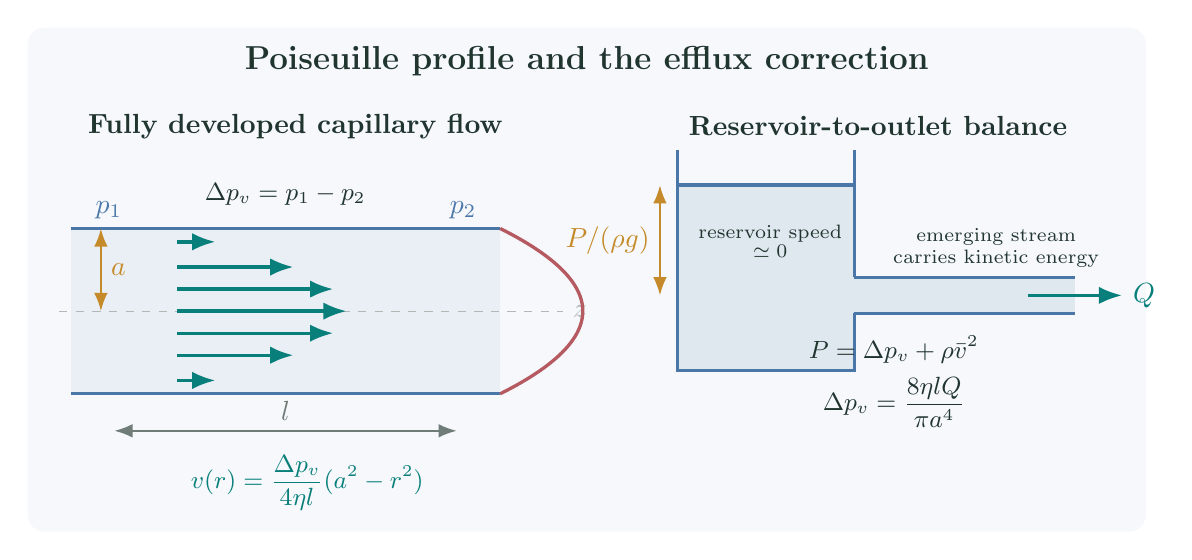
\begin{tikzpicture}[font=\sffamily,text=ink,>=Latex]
  \fill[blue!5,rounded corners=6pt] (-7.1,-3.15) rectangle (7.1,3.25);
  \node[font=\bfseries\large] at (0,2.82)
    {Poiseuille profile and the efflux correction};

  \begin{scope}[shift={(-6.55,-.35)}]
    \node[font=\bfseries] at (2.85,2.35) {Fully developed capillary flow};
    \fill[blue!12] (0,-1.05) rectangle (5.45,1.05);
    \draw[blue,very thick] (0,1.05)--(5.45,1.05);
    \draw[blue,very thick] (0,-1.05)--(5.45,-1.05);
    \draw[ink!35,dashed] (-.15,0)--(6.25,0) node[right] {$z$};
    \node[blue,above] at (.48,1.05) {$p_1$};
    \node[blue,above] at (4.98,1.05) {$p_2$};
    \draw[<->,gold,thick] (.38,0)--(.38,1.05) node[midway,right] {$a$};
    \draw[<->,ink!65,thick] (.55,-1.52)--(4.90,-1.52)
      node[midway,above] {$l$};
    \node[font=\small] at (2.72,1.48) {$\Delta p_v=p_1-p_2$};

    \foreach \y in {-.88,-.56,-.28,0,.28,.56,.88} {
      \pgfmathsetmacro{\len}{2.15*(1-\y*\y)}
      \draw[teal,very thick,->] (1.35,\y)--++(\len,0);
    }
    \draw[rose,very thick,domain=-1.05:1.05,samples=70]
      plot ({5.45+1.05*(1-(\x/1.05)^2)},\x);
    \node[teal,align=center,font=\small] at (3.00,-2.18)
      {$\displaystyle v(r)=\frac{\Delta p_v}{4\eta l}(a^2-r^2)$};
  \end{scope}

  \begin{scope}[shift={(1.15,-1.10)}]
    \node[font=\bfseries] at (2.55,3.10) {Reservoir-to-outlet balance};
    \fill[blue!18] (0,0) rectangle (2.25,2.35);
    \draw[blue,very thick] (0,2.8)--(0,0)--(2.25,0)--(2.25,.72);
    \draw[blue,very thick] (2.25,1.18)--(2.25,2.8);
    \draw[blue,very thick] (0,2.35)--(2.25,2.35);
    \fill[blue!18] (2.25,.72) rectangle (5.05,1.18);
    \draw[blue,very thick] (2.25,.72)--(5.05,.72);
    \draw[blue,very thick] (2.25,1.18)--(5.05,1.18);
    \draw[teal,very thick,->] (4.45,.95)--(5.65,.95)
      node[right] {$Q$};
    \draw[<->,gold,thick] (-.22,.95)--(-.22,2.35)
      node[midway,left] {$P/(\rho g)$};
    \node[font=\scriptsize,align=center] at (1.18,1.64)
      {reservoir speed\\[-1pt]$\simeq0$};
    \node[font=\scriptsize,align=center] at (4.05,1.55)
      {emerging stream\\carries kinetic energy};
    \node[align=center,font=\small] at (2.75,-.15)
      {$\displaystyle P=\Delta p_v+\rho\bar v^2$\\[4pt]
       $\displaystyle \Delta p_v=\frac{8\eta lQ}{\pi a^4}$};
  \end{scope}
\end{tikzpicture}
\end{document}
